\documentclass	[11pt, a4paper, openany]{book}
\usepackage[utf8]{inputenc}
\usepackage[francais]{babel}
\usepackage[T1]{fontenc}
\usepackage{amsmath}
\usepackage{amsfonts}
\usepackage{amssymb}
\usepackage{lmodern}
\usepackage{amsthm}

\usepackage{graphicx} % ajout image
\usepackage[tt]{titlepic}%Centre le titre

\usepackage{shorttoc} %Permet d'avoir de petites tables des matières


\usepackage{shapepar} %texte en keur
\usepackage{siunitx} %S.I.

\usepackage{graphicx}
\usepackage{caption} %Permet d'ajouter des légendes en images sans les mettre en float + ds la marge
\usepackage{delarray} % Belles matrices

\usepackage{fancyhdr} %Permet de modifier l'entête & footer
\usepackage{bbding} % Note marge
\usepackage{todonotes}
\usepackage{wrapfig}

\pagestyle{headings} % Titre du ch et numéro page dans l'entete
\usepackage{fullpage} %Utilise toute la page




\newcommand{\cst}{\text{cst}}
\newcommand{\E}{\vec E}
\newcommand{\F}{\vec F}

\newcommand{\questpm}[3]{#1. \textbf{#3} (p.#2)}
\newcommand{\exerc}[2]{\textbf{\Large Exercice #1\normalsize \\#2}}
\newcommand{\dif}{\mathrm{d}}
\newcommand{\comment}[1]{}
\newcommand{\rot}{\text{rot}\,}
\newcommand{\divv}{\text{div}\,}
\newcommand{\phas}[1]{\underline{#1}}
\newcommand{\RE}{\text{Re}}
\DeclareMathOperator{\arccot}{arccot}
\newcommand{\com}[1]{}

%\newcommand{\oiint}{\int\!\!\!\!\!\:\!\!\!\;\!\!\subset\!\!\supset\!\!\!\:\!\!\!\!\!\int}
\newcommand{\oiint}{\int\!\!\!\!\!\!\! \:\!\subset\!\!\supset\!\!\!\!\!\!\!\int}



\begin{document}
\renewcommand{\proofname}{Démonstration}
\frontmatter
\begin{titlepage}
\begin{center}	
	
	\newcommand{\HRule}{\rule{\linewidth}{0.5mm}}   			%Titre en gros
	
\includegraphics[scale=0.11]{logo.jpg}~\\[1cm]				%Logo

	\textsc{\LARGE Université Libre de Bruxelles}\\[1.5cm]
	\textsc{\Large Synthèse}\\[0.5cm]

	\HRule \\[0.4cm]
	{ \huge \bfseries Physique générale \\[0.4cm] }


	\HRule \\[1.5cm]
		\begin{minipage}{0.4\textwidth}
		\begin{flushleft} \large
		
		\emph{Auteur:}\\
			Nicolas \textsc{Englebert}\\
			\end{flushleft}
			\end{minipage}
			\begin{minipage}{0.4\textwidth}
			\begin{flushright} \large
			\emph{} \\		
			\textsc{}
			\end{flushright}
		\end{minipage}

	\vfill

% Bottom of the page
{\large \today}

\end{center}
\end{titlepage}





\part{Introduction}
\chapter{A propos du document}
A




\mainmatter
\part{Synthèse du cours}
\chapter{Thermodynamique}
\section{Introduction}
Une brève introduction aux degrés de libertés. Une lecture attentive suffira.

\section{La pression}

\begin{wrapfigure}[10]{l}{4cm}
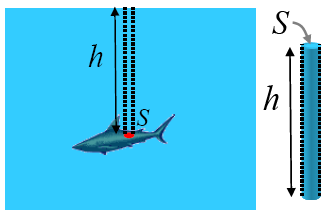
\includegraphics[width=4cm]{th/image1.png}
\captionof{figure}{Pression hydrostatique}
\end{wrapfigure}

Dans notre cas, le poids est la force engendrée par la colonne d'eau. Comme celle-ci est liquide, sont poids vaut $\underbrace{\rho V}_m  g$.\\
Par définition, de la pression : $P \equiv \frac{Poids}{Surface}$ on peut trouver la pression hydrostatique \footnote{Que pour des liquides incompressibles} :
\begin{equation}
\fbox{$P_{hydrostatique} = \rho g h $}
\end{equation}
Les unités de la pression sont les Pascals $\left(Pa = \dfrac{N}{m^2}\right)$. Notons également que 1 bar = $10^5\ Pa$ et que $1\ atm = 1,013\ bar$.

\subsection{Le baromètre}
\begin{wrapfigure}[10]{r}{3cm}
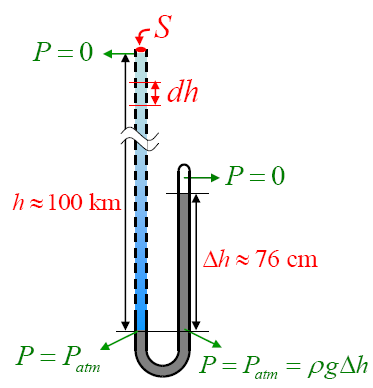
\includegraphics[scale=0.3]{th/image2.png}
\captionof{figure}{Baromètre}
\end{wrapfigure}
Son but est de mesurer la pression atmosphérique. La colonne d'air au dessus de nous à une hauteur de 100km. Si l'air était du mercure, cette colonne ferait 76mm de hauteur. \\

Ici l'air n'est pas un liquide incompressible, il faut donc passer par le formalisme intégral : 
\begin{equation}
Poids\ =\ \rho_{air}.g.s.dh
\end{equation}
Connaissant la définition de la pression, on peut calculer celle-ci
\begin{equation}
\int_0^h \frac{\rho_{air}g.S.dh}{S} = \rho_air.g.\Delta h
\end{equation}

\section{La température}
\subsection{Dilatation thermique}
Utilisation de la dilatation dans les thermomètres (Même si aujourd'hui on utilise de l'alcool, initialement c'était avec un gaz).

\subsection{Température absolue}
A l'aide d'un thermomètre à gaz à volume constant, \textit{Amontons} a mis en évidence une relation linéaire entre la pression et la température.
\begin{center}
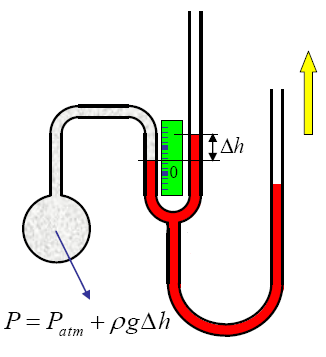
\includegraphics[scale=0.15]{th/image3.png}
\captionof{figure}{Thermomètre à gaz à volume constant}
\end{center}
\begin{equation}
P = \alpha T + P_0
\end{equation}
où $P_0$ est la température à $0 deg. C$.\\
En extrapolant les résultats par une série de mesure répétitive, \textit{Amontons} a pu mettre en évidence l'existence du zéro absolu (-273,15 deg. C)
\begin{center}
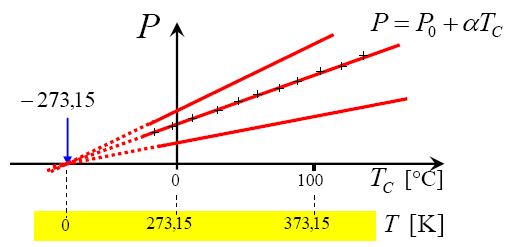
\includegraphics[scale=0.3]{th/image4.png}
\captionof{figure}{Extrapolation du zéro absolu}
\end{center}

\section{Comportement des gaz}
\subsection{Loi de Gay-Lussac (Amontons)}
Cette loi est la même que celle découverte par \textit{Amontons}. Elle dit que la pression est proportionnelle à la température à volume constant.
\begin{equation}
P \propto T|_{V = cste}
\end{equation}

\subsection{Loi de Charles}
\begin{wrapfigure}[7]{l}{3cm}
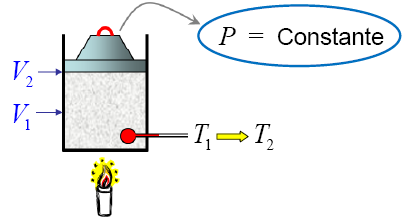
\includegraphics[scale=0.23]{th/image5.png}
\captionof{figure}{Loi de Charles}
\end{wrapfigure}
Par le placement d'un poids libre de se mouvoir, la pression est maintenue constante. Ceci permis l'étude de l'élévation du piston à pression constante et de dériver la Loi de Charles :
\begin{equation}
V \propto T|_{P = cste}
\end{equation}

\subsection{Loi de Boyle et Mariotte}
Ces deux scientifiques ont mis en évidence une relation entre le volume et la pression à température constante :
\begin{equation}
PV = cste|_{T = cste}
\end{equation}

\subsection{Loi des gaz parfaites}
En rassemblant les trois lois obtenues ci-dessus, on obtient : 
\begin{equation}
PV = \alpha T
\end{equation}
Si l'on devait doubler le nombre de particules de gaz, la constante $\alpha$ serait proportionnelle au nombre de particules multiplié par une constante ($\alpha \propto N.cste$).\\
Pour des raisons détaillée ci-dessous, $\alpha = N.k_B$ de la sorte que
\begin{equation}
\fbox{$ PV = N.k_BT$}
\end{equation}

\subsection{Loi d'Avogadro}
Le but est de déterminer la valeur de la \textit{constante de Boltzman}, $k_B$ grâce à la loi d'Avogadro : Si la pression et la température sont constantes, la volume $V$ occupé par $N$ particules est le même.\\ Ce n'est donc pas le nombre d'atomes qui détermine le volume. En isolant $V$ :
\begin{equation}
V = k_B . \frac{NT}{P}
\end{equation}
Or, $\frac{NT}{P}$ donnant une valeur unique pour un gaz, $k_B$ est une constante universelle. \\En posant $P=1atm, T = 237,15K, V = 22,4 L$ on trouve :
\begin{equation}
k_B = 1,38.10^{-23}\ \frac{Pa.m^3}{K}\ \ \  \left(= \frac{N.m^3}{m^2.K} = \frac{J}{K}\right)
\end{equation}

\subsection{Constante universelle des gaz parfaits}
Le nombre de moles étant donné par $n = N/N_A$, on déduit que $N = n.N_A$. En substituant dans la loi des gaz parfaits\footnote{Valabie si $P$ pas trop grande et $T$ pas trop petite} :
\begin{eqnarray}
PV &=& n.\underbrace{N_A.k_B}_R T\\
PV &=& nRT
\end{eqnarray}
où $R\ =\ 8,314\ J/K$.

\section{Théorie cinétique des gaz parfaits}
Un gaz est un ensemble de particules en mouvement incessant (dit parfait s'il $\nexists$ d'interactions entres particules). Chaque particule cause un impact générant une pression.
\begin{equation}
Force\ d'impact\ : f = m\frac{dv}{dt}
\end{equation}

\subsection{Incidence normale}
Lors d'un impact, la particule s'écrase et regagne une accélération.
\begin{center}
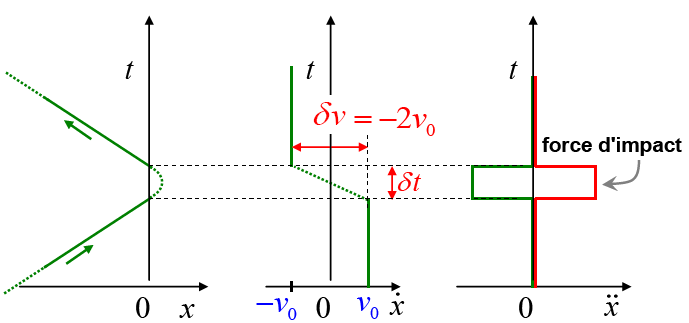
\includegraphics[scale=0.4]{th/image6.png}
\captionof{figure}{Incidence normale : Position - Vitesse - Accélération}
\end{center}
En prenant l'hypothèse que l'accélération est constante $\ddot{x} = a = cste$ on peut trouver la vitesse par intégration  : $\dot{x} = at + C$.\\
Grâce à $f = ma$, on peut calculer la force d'impact (on suppose $dv/dt = \partial v / \partial t$ (hypoth. de modél.comme $V = cste$)) sachant que la vitesse vaut = $v = -v_0 - v_0 = -2v_0$ (voir schéma ci-dessus)
\begin{equation}
f = m\ddot{x} = m\frac{dv}{dt} = m\frac{\partial v}{\partial t} = -m\frac{2v_0}{\partial t}
\end{equation}
Comme $\overline{f_i} = -f$, la force d'impact moyenne vaut :
\begin{equation}
\overline{f_i} = m \frac{2v_0}{\partial t}\vec{1_x}
\end{equation}
Le signe est positif car la force se dirige vers les $x > 0$  (Action/réaction)

\subsection{Incidence oblique}
Cela ne change rien, il suffit de considérer une vitesse vectorielle pour s'en rendre compte
\begin{equation}
\vec v = v_x \vec{1_x} + v_y \vec{1_y} + v_z \vec{1_z}
\end{equation}
Comme seule la composante en $x$ varie, nous retrouverons bien le résultat précédent 
\begin{equation}
f_i = m\frac{2v_x}{\partial t}
\end{equation}

\subsection{Force d'impact périodique}
\begin{wrapfigure}[7]{l}{3cm}
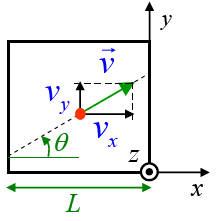
\includegraphics[scale=0.4]{th/image7.png}
\captionof{figure}{Aller/retour}
\end{wrapfigure}
On veut connaître le temps d'un aller-retour. Connaissant la formule du MRU $d = vt \Rightarrow t = \frac{d}{v}$.
$\\
\left\{\begin{array}{l}
d = L\\
v = v_x = v.\cos\theta
\end{array}\right.
$ \ \ \ $\Rightarrow \Delta t = \dfrac{L}{v.\cos\theta}$
Comme nous nous intéressons à un aller/retour, il convient de considérer une longueur double :
\begin{equation}
\Delta t = \frac{2L}{v_x}
\end{equation}
\subsection{Force continue}
Il y a beaucoup de particules : impossible de tous les traiter individuellement. On va alors passer au concept de la \textit{force continue}.

\subsection{Force d'impact moyenne}
Comment éliminer $\delta t$ (le temps du choc) ? On imagine qu'une particule tape périodiquement sur un piston.
\begin{itemize}
\item Le piston monte : $(f - mg)$
\item Le piston descend (entre impact) : $(-mg)$
\end{itemize}
Dans une position d'équilibre ou le poids sur le piston reste fixe, la gravité contre parfaitement la montée du piston 
\begin{equation}
g = f_i - mg
\end{equation}
On étudiant les extrêmes, on peut trouver la vitesse moyenne nulle, c'est à dire une position d'équilibre.\\
$\left\{\begin{array}{l}
Variation\ totale\ v = at  \Rightarrow \dfrac{1}{M}\left(f_i - Mg\right)\delta t\\
Variation\ pensenteur\ seule  \Rightarrow g(\Delta t -  \delta t)
\end{array}\right.$\\
En considérant la situation d'équilibre
\begin{eqnarray}
\frac{1}{M}(f_i - mg)\delta t &=& g(\Delta t - \delta t)\\
(f_i - mg)\delta t &=& mg(\Delta t - \delta t)\\
f_i\Delta t - mg\delta t &=& - mg\delta t + mg \Delta t\\
f_i \delta t &=& Mg\Delta t
\end{eqnarray}
Cette dernière équation traduit que l'action de la force d'impact sur un temps $\delta t$ équilibre la gravité sur le temps $\Delta t$.\\

Le piston étant à l'équilibre, on peut dire que sa force d'impact moyenne $\overline{f_i} = Mg$. On peut voir ceci comme la force que je dois appliquer pour lever le piston, la force moyenne à fournir.  On a donc (Sur base de la dernière équation)
\begin{equation}
\overline{f_i} = f_i \frac{\delta t}{\Delta t}
\end{equation}
où $f_i$ est la force intermittente.

\subsection{Force totale}
$\left\{\begin{array}{l}
f_i = m\dfrac{2v_x}{\delta t}\\
\overline{f_i} = fi\dfrac{\delta t}{\Delta t}
\end{array}\right.$\ \ \ $\Rightarrow \overline{f_i} = m\dfrac{2v_x}{\delta t}\frac{\delta t}{\Delta t}\ \ \ \Rightarrow \overline{f_i} = m\frac{2v_x}{\Delta t}$\\
Connaissant $\Delta t = 2L/v_x$, on trouve : 
\begin{equation}
\overline{f_i} = \frac{mv_x^2}{L}
\end{equation}
Pour $N$ particules (On multiplie et divise par $N$ pour faire apparaître la moyenne)
\begin{equation}
F_{tot} = \sum \frac{mv_x^2}{L} = \frac{Nm}{L}<v_x^2>
\end{equation}
$F_{tot}$ représente l'ensemble des force sur une période. On considérant les vitesses $v_x, v_y$ et $v_z$ isotropes :
\begin{equation}
<v^2> = <v_x^2> + <v_y^2> + <v_z^2>\ \ \ \ \ \ \ \ \Rightarrow \ \ \ <v_x^2> = \frac{1}{3}<v^2>
\end{equation}
Nous trouvons ainsi notre expression finale de la force totale 
\begin{equation}
f_{tot} = \frac{Nm}{3M}<v^2>
\end{equation}
\subsection{Calcul de la pression}
En se basant sur la définition de la pression
\begin{equation}
P = \frac{Nm}{3\underbrace{SL}_V}<v^2>\ \ \ \ \ \Rightarrow \ \ \ \ \ PV = \frac{Nm<v^2>}{3}
\end{equation}
\subsection{Théorie - expérience}
En égalant l'expression obtenue ci-dessus avec $PV = Nk_BT$, on peut retrouver l'expression de la température
\begin{equation}
T = \frac{m<v^2>}{3k_B}
\end{equation}
On retrouve implicitement l'expression de l'énergie cinétique, nous permettant de ré-écrire cette expression de la sorte
\begin{equation}
\fbox{$ T = \frac{2E_{cin}}{3k_B}$}
\end{equation}
Ceci démontre de façon formelle que la température est bien proportionnelle à l'énergie cinétique des particules.

\section{L'énergie thermique}
On va appeler l'énergie interne d'un gaz $U$ la somme de toutes les énergie cinétique d'un gaz. Sachant que $T = \dfrac{2E_{cin}}{3k_B}$ :
\begin{equation}
\fbox{$ U = N.E_{cin} = \frac{3}{2}Nk_BT$}
\end{equation}


\subsection{Expérience de Joule}
En faisant bouger de l'eau, on augmente son énergie cinétique causant une augmentation de la température $\Rightarrow$ augmentation de l'énergie interne, $U$.

\subsection{Échauffement et chaleur}
L'échauffement est un transfert \textit{collisionnel} d'énergie cinétique désordonnée. La chaleur \textbf{transmise} se note $Q\ [J]$.

\subsection{Équilibre thermique}
La propagation par transfert collisionnel homogène du aux mouvements erratiques se nomme l'\textit{équipartition}. Il conduit à une uniformisation de la température et défini le \textbf{Premier principe de la thermodynamique}
\begin{center}
\fbox{\textit{\textsc{Principe zéro :} équipartition de l'énergie thermique.}}
\end{center}

\subsection{Capacité calorifique}
Il s'agit de la quantité de chaleur apportée $Q$ sur la variation de température 
\begin{equation}
\Delta T : C_V = \dfrac{Q}{\Delta T}|_{v=cste} = \frac{3}{2}Nk_B
\end{equation}
Il faut $12.5J$ pour chauffer une mole de gaz \textbf{monoatomique} de $1K$.

\subsection{Gaz polyatomique}
Il y a plus de degré de liberté pour ce type de gaz. Il faudra dès lors plus de chaleur pour chauffer une mole de gaz car cette énergie ira à l'énergie de rotation, de vibration et de translation. En effet :
\begin{equation}
U \equiv N.E_{cin} + N.E_R + N.E_V
\end{equation}
Pour tenir compte de ce plus grand nombre de degré de liberté, il suffit d'utiliser cette expression :
\begin{equation}
U = \frac{n_d}{2}Nk_BT\ \ \ \ où \ \left\{\begin{array}{l}
n_d = 3 \ \ \ (gaz\ monoatomique)\\
n_d = 7 \ \ \ (gaz\ polyatomique)
\end{array}\right.
\end{equation}
Compte-tenu de ce résultat, la capacité \textit{molaire} à volume constant aura pour expression :
\begin{equation}
\fbox{$ C_V = \frac{n_d}{2}R$}
\end{equation}

\subsection{Capacité calorifique massique}
Par définition :
\begin{equation}
\fbox{$ Q \equiv c_v m \Delta T$}
\end{equation}
où $c_v$ est la quantité de chaleur nécessaire à l'élévation de $1K, 1kg$ de gaz à volume constant.
\begin{equation}
c_v = \frac{n_d}{2}\frac{R}{M_m}\ \ \ \left(\left[\frac{J}{kg.K}\right]\right)
\end{equation}

\subsection{Capacité calorifique de l'eau}
Il faut $4186\ J$ pour augmenter de $1\ K$ un kilogramme d'eau de 14.5 à 15.5 degré celsius.\\
On définit ainsi $1\ cal = 4.186J$ d'où $1\ kcal = 4186J$.
\begin{equation}
c_{H_2O} = 4186\ \frac{J}{kg.K}
\end{equation}
La grande capacité de l'eau est du à sa polarité : briser ses liaisons demande une énergie plus importante (Plus une capacité est grande, plus le $\Delta T$ sera en effet faible).

\subsection{Mécanisme de transfert de l'énergie thermique}
\subsubsection{La conduction}
\begin{wrapfigure}[11]{l}{3cm}
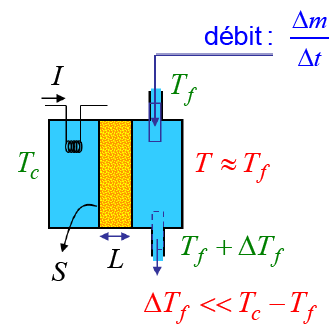
\includegraphics[scale=0.4]{th/image8.png}
\captionof{figure}{Conductivité thermique}
\end{wrapfigure}
\textit{Fourrier} a mis en évidence que le tranfert collisionnel est du à l'agitation thermique. Il a créé un dispositif permettant de connaître la capacité calorifique des matériaux grâce à la connaissance de celle de l'eau.\\

Pour se faire, il a fait un \textbf{bilan énergétique} : on regarde ce qui entre et ce qui sort sur un temps $\Delta t$. On notera $H$ la quantité de chaleur transférée par conduction par unité de temps. On remarque expérimentalement :\\
$\left\{\begin{array}{l}
H \propto \Delta T\\
H \propto S\\
H \propto \dfrac{1}{L}
\end{array}\right.$\\
On introduit dès lors une constante de proportionnalité, $k_T$ comme étant la \textit{conductivité thermique}.
\begin{equation}
\fbox{$ H = k_TS\frac{\Delta T}{L}$}
\end{equation}

\section{Transformations thermodynamiques}
\subsection{Système thermodynamique}
\subsubsection{Premier principe de la thermodynamique}
\begin{wrapfigure}[6]{r}{5cm}
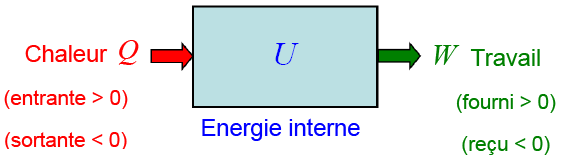
\includegraphics[scale=0.4]{th/image9.png}
\captionof{figure}{Premier principe}
\end{wrapfigure}
Le premier principe de la thermodynamique se base sur la conservation de l'énergie, la quantité totale d'énergie n'est jamais modifiée.\\
\begin{center}
\fbox{\textsc{Premier principe :} $\Delta U = Q - W$}
\end{center}
La production d'un travail épuise l'énergie interne. On ne peut avoir un travail infini car la chaleur $Q$ ne l'est pas.\\
Tout système violant ce principe portera le doux nom de \textit{machine à mouvement perpétuel de première espèce.}

\subsection{État d'un système et transformation}
On utilise des variables d'état pour caractériser un gaz ($P, V, T, N$).

\subsection{La transformation isobare}
\begin{wrapfigure}[8]{l}{5cm}
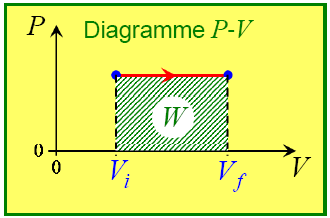
\includegraphics[scale=0.34]{th/image10.png}
\captionof{figure}{Isobare}
\end{wrapfigure}
Il s'agit d'une transformation à pression constante. Le volume du gaz se verra modifié suite à une modification de la température. \\
Le calcul du travail est simple car la pression est constante 
\begin{equation}
W_{isobare} = F.\Delta L = P. \Delta V
\end{equation}
Quel est la relation entre $Delta T$ et $W$ ?\\
$\left\{\begin{array}{l}
T_i =  \frac{P}{Nk_B}V_i\\
T_f = \frac{P}{Nk_B}V_f\\
T_i - T_f = \Delta T
\end{array}\right.$\ \ \ \ \ $\Rightarrow\ \ \Delta T = \frac{P}{Nk_B}\Delta V = \frac{W}{Nk_B}$.

\subsubsection{Bilan détente isobare}
On sait : $\left\{\begin{array}{l}
W = P\Delta V\\
\Delta U = Q - W\\
Gaz\ parfait\ : \Delta U = \frac{n_d}{2}Nk_B\Delta T\\
\Delta T = \frac{W}{Nk_B}
\end{array}\right.$ d'où on tire : $Q = \frac{n_d}{2}W + W = W(\frac{n_d}{2}+1)$\\
Le rendement vaut donc 
\begin{equation}
r = \frac{W}{Q} = \frac{1}{1 + \frac{n_d}{2}}
\end{equation}

\subsubsection{Capacité calorifique molaire à pression constante}
Par définition 
\begin{equation}
Q \equiv C_p n \Delta T
\end{equation}
Que vaut $C_p$? Nous savons que $Q = \Delta U + P\Delta V \Rightarrow \frac{Q}{\Delta T} = \frac{\Delta U}{\Delta T} + \frac{P\Delta V}{\Delta T} \equiv C_p (1)$\\
Or $U = \frac{n_d}{2}RT \rightarrow \Delta U = \frac{n_d}{2}R\Delta T (2)$.\\
On réinjectant (2) dans (1), nous trouvons l'expression de la capacité molaire à pression constante.
\begin{equation}
C_p = \frac{n_d}{2}R + R = R(\frac{n_d}{2}+1)
\end{equation}
On remarque que, pour un gaz parfait, $C_p - C_v = R$. $C_p > C_v$ car il y a un travail mécanique à fournir en plus.


\subsection{La transformation isochore}
\begin{wrapfigure}[8]{l}{4cm}
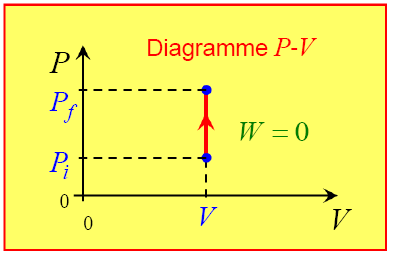
\includegraphics[scale=0.24]{th/image11.png}
\captionof{figure}{Isochore}
\end{wrapfigure}
Caractérisée par un volume constant : $\Delta V = 0 \Rightarrow W = 0$.\\
Différence de température $T$ pour une chaleur $Q$ fournie ? Sachant que $Q = \Delta U + W$ où $W = 0$, on sait que $Q = \frac{n_d}{2}nR\Delta T$\footnote{On travaille avec des moles ($n$) ici !}.\\Nous avons donc :
\begin{equation}
\Delta T = \frac{2Q}{n_d Rn}
\end{equation}

\subsubsection{Travail d'une transformation quelconque}
\begin{wrapfigure}[8]{r}{3cm}
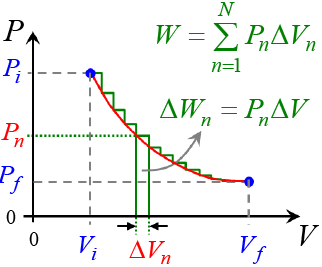
\includegraphics[scale=0.34]{th/image12.png}
\captionof{figure}{Transformation quelconque}
\end{wrapfigure}
L'expression du travail d'une transformation quelconque peut être vue approchée comme étant une suite d'isobare ($W = P\Delta V$) et d'isochore ($W = 0$) : $W = \sum P_n \Delta V_n$\\ En faisant tendre $\Delta V \rightarrow 0$ on retrouve la définition de l'intégrale (intégrale de circulation de la force transmise par le gaz)
\begin{equation}
W = \int_{V_i}^{V_f} P(V).dV
\end{equation}
\subsection{La transformation isotherme}
Il s'agit d'une transformation dite \textit{idéale}. Elle se base sur l'hypothèse de la présence d'une paroi mince et d'une transformation \textbf{lente} : le gaz à toujours la même température. 
\begin{center}
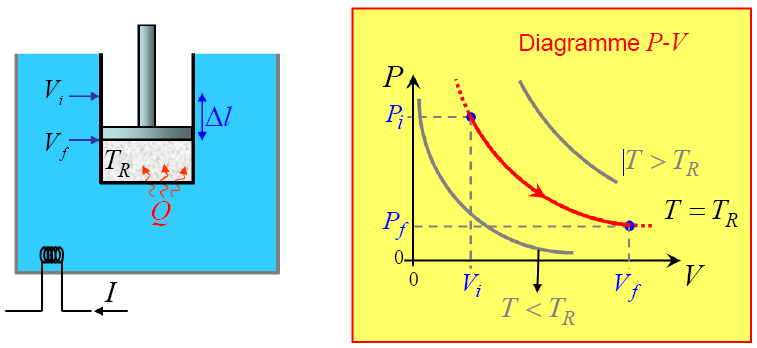
\includegraphics[scale=0.3]{th/image13.png}
\captionof{figure}{Exemple de transformation isotherme (gauche) et son diagramme PV (droite)}
\end{center}
Si l'on lève le piston de $\Delta l$ le volume augmente et comme $PV=cste$, la pression va diminuer.\\
Intuitivement, en levant le piston on \textit{amorti} les particules causant une diminution de la pression et de la température (comme l'$E_{cin}$ diminue).

\subsubsection{Bilan énergétique de la transformation isotherme}
Calculons tout d'abord le travail de cette transformation à l'aide de la relation obtenue ci-dessus ($T_r$ = température du réservoir).
\begin{equation}
W = \int_{V_i}^{V_f} P(V).dV\ \ où\ \ P = \frac{Nk_BT_r}{V}
\end{equation}
Après intégration, nous trouvons le travail d'une isotherme
\begin{equation}
W_{isoth} = Nk_BT_r \ln\left(\frac{V_f}{V_i}\right)
\end{equation}
Il n'y a pas de différence de température ($\Delta T = 0$) dans cette transformation $\Rightarrow \Delta U = \frac{n_d}{2}Nk_B\Delta T = 0$.\\
Dans une transformation isotherme $Q = W$ : le rendement est dès lors maximum.
\begin{equation}
r = \frac{W}{Q} = 1
\end{equation}

\subsection{La transformation adiabatique}
A l'inverse de la transformation isotherme, celle-ci se déroule \textbf{sans} échange de chaleur : $Q = 0$. C'est \textit{Pierre-Simon Laplace} qui a trouvé qu'il existe une relation particulière en l'absence d'échange de chaleur. Son génie est d'être passé par la décomposition infinitésimale.
\begin{eqnarray}
dU &=& dQ - dW\ \ \ où\ \ dQ = 0\\
  &=& - dW \ \ \ \ où\ \ dU = \frac{n_d}{2}Nk_B dt = - PdV
\end{eqnarray}
Sachant que (Loi des gaz parfaits) $P = \dfrac{Nk_BT}{V}$ on peut écrire 
\begin{eqnarray}
\frac{n_d}{2}Nk_Bdt = - \frac{Nk_BT}{V}dV\\
\frac{n_d}{2}\frac{dT}{T} = - \frac{dV}{V}
\end{eqnarray}
On intégrant de part et d'autres
\begin{eqnarray}
\int_{T_i}^{T} \frac{dT}{T} &=& -\frac{2}{n_d}\int_{V_i}^{V} \frac{dV}{V}\\
\ln\left(\frac{T}{T_i}\right) &=& -\frac{2}{n_d}\ln\left(\frac{V}{V_i}\right)\\
\ln\left(\frac{T}{T_i}\right) &=& \ln\left(\frac{V}{V_i}\right)^{-\frac{2}{n_d}}\\
\frac{T}{T_i} &=& \left(\frac{V_i}{V}\right)^{\frac{2}{n_d}}\\
TV^{\frac{2}{n_d}} &=& T_iV_i^{\frac{2}{n_d}}
\end{eqnarray}
On en tire ce que l'on appelle la \textit{Loi de Laplace}
\begin{equation}
TV^{\frac{2}{n_d}}\ =\ cste
\end{equation}

\subsubsection{Diagramme PV de la transfo adiabatique}
\begin{wrapfigure}[8]{r}{3cm}
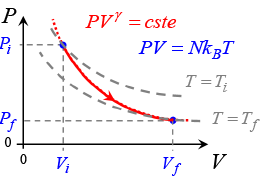
\includegraphics[scale=0.44]{th/image14.png}
\captionof{figure}{Adiabatique}
\end{wrapfigure}
Pour pouvoir tracer le diagramme PV, il faut ré-exprimer la loi de Laplace en fonction de $P$ et $V$. Sachant que : \\
$\left\{\begin{array}{l}
TV^{\frac{2}{n_d}}\ =\ cste\\
T = \dfrac{PV}{Nk_B}
\end{array}\right.$\ \ \ \ $\Rightarrow \frac{PV}{Nk_B}V^{\frac{2}{n_d}} = cste$\\
Ce que l'on peut ré-écrire $PV^{1 + \frac{2}{n_d}} = cste$. En posant $(1 + \frac{2}{n_d}) = \gamma$ (coefficient adiabatique) :
\begin{equation}
\fbox{$PV^\gamma = cste$}
\end{equation}
\newpage
\section{Les cycles thermodynamiques}
\begin{wrapfigure}[9]{r}{3cm}
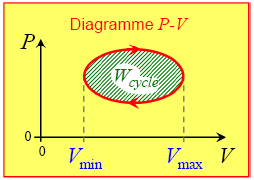
\includegraphics[scale=0.44]{th/image15.png}
\captionof{figure}{Cycle thermo}
\end{wrapfigure}
Un cycle thermodynamique est une suite de transformations formant un cycle dans l'espace des variables d'état. Le travail d'un cycle se défini de la sorte :
\begin{equation}
W_{cycle} = \oint P(V).dV
\end{equation}
Tout ce qui est gagné dans un cycle est perdu à un autre moment. Dès lors 
\begin{equation}
\Delta U_{cycle} = Q_{cycle} - W_{cycle} \equiv 0
\end{equation}
\subsection{Le cycle de Carnot}
\begin{wrapfigure}[6]{l}{5cm}
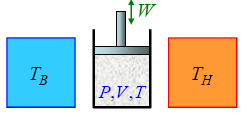
\includegraphics[scale=0.64]{th/image16.png}
\captionof{figure}{Machine de Carnot}
\end{wrapfigure}
Il s'agit d'une machine idéale divisée en 4 étapes :
\begin{enumerate}
\item Détente isotherme $T_H$
\item Détente adiabatique
\item Compression isotherme $T_B$
\item Compression adiabatique
\end{enumerate}
\ \\
\begin{wrapfigure}[1]{r}{5cm}
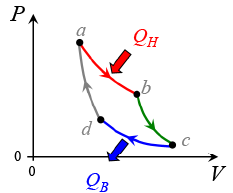
\includegraphics[scale=0.54]{th/image17.png}
\captionof{figure}{Cycle de Carnot}
\end{wrapfigure}
\subsubsection{Détente isotherme}
$\left\{\begin{array}{l}
W_{ab} = \int P(V)dV \rightarrow W_{ab} = Nk_BT_H\ln\left(\frac{V_b}{V_a}\right)\\
\Delta U = 0
\end{array}\right.$

\subsubsection{Détente adiabatique}
On déconnecte de $T_H$ mais ça monte encore un petit peu (comme par "inertie")\\
$\left\{\begin{array}{l}
\Delta U_{bc} = \frac{n_d}{2}Nk_B(T_H-T_B)\\
W_{bc} = \frac{Nk_B}{\gamma - 1}(T_H - T_B)
\end{array}\right.$

\subsubsection{Compression isotherme}
$\left\{\begin{array}{l}
W_{ab} = Nk_BT_B\ln\left(\frac{V_d}{V_c}\right)\\
\Delta U = 0
\end{array}\right.$

\subsubsection{Compression adiabatique}
$\left\{\begin{array}{l}
W_{bc} = \frac{Nk_B}{\gamma - 1}(T_B - T_H)\\
\Delta U = - W_{da}
\end{array}\right.$

\subsubsection{Bilan énergétique du moteur de Carnot}
Ceci est très algébrique et se trouve dans le syllabus. Seul le résultat final est exposé ici (la démo est à connaître pour l'examen!!) :
\begin{eqnarray}
W_{carnot} = Nk_B\ln\left(\frac{V_b}{V_a}\right).\left[T_H - T_B\right]\\
Q_B = -\frac{T_B}{T_H}Q_H
\end{eqnarray}


\subsubsection{Rendement du cycle de Carnot}
\begin{equation}
r_c = 1 - \frac{T_B}{T_H}
\end{equation}
Ceci montre que si la température du réservoir froid tend vers zéro kelvin, on tend vers un rendement maximal.


\subsection{Le moteur à combustion interne}
\begin{wrapfigure}[9]{r}{4cm}
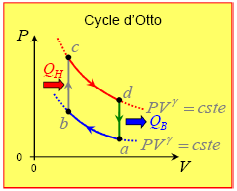
\includegraphics[scale=0.54]{th/image18.png}
\captionof{figure}{Cycle d'Otto}
\end{wrapfigure}
Connu sous le nom du cycle d'\textit{Otto}, ce-dernier se compose de quatre étapes :
\begin{itemize}
\item[AB] Adiabatique (montée rapide du piston)
\item[BC] Isochore (Explosion)
\item[CD] Adiabatique (détente)
\item[DA] Isochore (refroidissement)
\end{itemize}
Encore une fois, seule les résultats finaux sont repris ici mais le développement est à connaître pour l'examen!!
\begin{eqnarray}
Q_B = -\left(\frac{V_b}{V_a}\right)^{\gamma -1}Q_H\\
r = \frac{W}{Q_H} = 1 - \frac{|Q_B|}{Q_H} = 1 - \left(\frac{V_b}{V_a}\right)^{\gamma -1}
\end{eqnarray}


\subsection{Le moteur à turbine à gaz (Cycle de Brayton)}
Le cycle se compose de quatre étapes (encore une fois je ne fais que citer, mais la flemme de recopier tous les dev' mathématiques!)
\begin{enumerate}
\item Gaz dans un cicuit fermé mis en circuit par un compresseur 
\item Gaz chauffé une fois compressé
\item Gaz détendu dans la turbine
\item Gaz refroidit
\end{enumerate}

\subsubsection{Le réfrigérateur (Cycle de Brayton inversé)}
Le principe est celui du moteur à turbine à gaz si ce n'est que c'est exactement l'inverse !
\begin{enumerate}
\item Gaz comprimé adiabatiquement
\item Gaz comprimé chaud refroidi dans un échangeur thermique
\item Gaz détendu de façon adiabatique
\item Le gaz refroidi se réchauffe en pompant la chaleur
\end{enumerate}

\newpage
\section{Entropie et second principe}
\subsection{Analyse de \textit{Clausius} avec le cycle de \textit{Carnot}}
\textit{Clausius} s'est intéressé à la relation particulière du cycle de Carnot.
\begin{equation}
r_c = 1 - \frac{|Q_B|}{Q_H} = 1 - \frac{T_B}{T_H}
\end{equation}
On peut en déduire la définition de l'entropie ; tout ce qui rentre, sort.
\begin{equation}
\frac{Q_B}{T_B} = -\frac{T_B}{T_H} \equiv Entropie
\end{equation}
On dira, dans ce cas, que l'entropie est conservée :
\begin{equation}
\fbox{$\frac{Q_B}{T_B} + \frac{Q_H}{T_H} = 0$}
\end{equation}

\subsection{Généralisation à tout cycle}
Il suffit de remplacer le cycle par une suite d'isotherme et d'adiabatique afin de retrouver $Q_B$ et $Q_H$.
\begin{equation}
\frac{\delta Q_H}{\delta T_H} + \frac{\delta Q_B}{\delta T_B} = 0
\end{equation}
En prenant la limite infinitésimale, on retrouve le résultat précédent sous sa forme intégrale
\begin{equation}
\fbox{$\Delta S =\oint \frac{dQ}{T} = 0$}
\end{equation}

\subsection{Définition de l'entropie}
\begin{wrapfigure}[7]{l}{4cm}
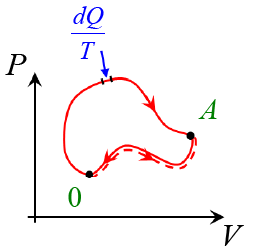
\includegraphics[scale=0.44]{th/image19.png}
\captionof{figure}{Cycle thermodynamique}
\end{wrapfigure}
Nous allons ici montrer que l'entropie est une \textbf{fonction d'état} : elle ne dépend que des états extrêmes.
\begin{eqnarray}
\oint \frac{dQ}{T} = 0 \Leftrightarrow \int_{0 \rightarrow A} \frac{dQ}{T} + \int_{A \rightarrow 0} \frac{dQ}{T} = 0\\
\int_{0 \rightarrow A} \frac{dQ}{T} = \int_{0 \rightarrow A} \frac{dQ}{T}
\end{eqnarray}
Ce qui est bien le résultat recherché : celui-ci est valable pour tout cycle.


\subsection{Moteurs et entropie}
L'entropie, $S(A)$ est nulle sur un cycle (tout comme $\Delta U$) :
\begin{equation}
W = \oint dW > 0\ \ \ \Rightarrow\ \ \ Q = \oint dQ > 0
\end{equation}
Il faut plus de chaleurs entrante que sortante sur le cycle d'un \textbf{moteur}. Ce n'est pas possible de ne pas rejeter $Q$ car sinon $\oint \frac{dQ}{T}$ ne serait pas nulle.\\
Si un moteur viole ceci, elle portera le nom de \textit{moteur à mouvement perpétuel de deuxième espèce.}

\subsection{Illustrations}
\subsubsection{Transformation isotherme}
\begin{equation}
\Delta Q = Nk_BT_r\ln\left(\frac{V_f}{V_i}\right)\ \ \ \ \ \ \ \Delta S_{isoth} = NK_b\ln\left(\frac{V_f}{V_i}\right)
\end{equation}

\subsubsection{Transformation adiabatique}
\begin{equation}
\Delta Q =0\ \ \ \ \ \ \ \Delta S_{adiab} = 0
\end{equation}

\subsubsection{Transformation isochore}
Attention, ici la température n'est pas constante ! Il faudra intégrer.
\begin{equation}
\Delta Q = \Delta U = \frac{n_d}{2}Nk_B\Delta T\ \ \ \ \ \ \ \Delta S_{isoc} = \Delta U = \frac{n_d}{2}Nk_B\int \frac{dT}{T}
\end{equation}
Ce qui nous donne
\begin{equation}
\Delta S_{isochore} = \frac{n_d}{2}Nk_B\ln\left(\frac{T_f}{T_i}\right)
\end{equation}


\subsubsection{Transformation isobare}
Le raisonnement est le même que pour l'isochore, mais on utilisera ici $C_p$ pour avoir le lien entre $Q$ et $T$ : $dQ = nC_p \Delta T$ où $C_p = (\frac{n_d}{2}+1)R$
\begin{equation}
\Delta S_{isobare} = \left(\frac{n_d}{2}+1\right)R\ln\left(\frac{T_f}{T_i}\right)
\end{equation}

\subsubsection{Cycle d'Otto}
Nous savons que l'entropie devra être nulle. Ici, il ne faut pas tenir compte des adiabatique mais juste des isochores (on les somme).
\begin{equation}
\Delta S_{Otto} = \frac{n_d}{2}Nk_B\left(\frac{T_cT_a}{T_bT_d}\right)
\end{equation}
En jouant avec la loi de Laplace des adiabatiques, on trouve que l'argument du $\ln$ vaut 1.
\begin{equation}
\Delta S_{Otto} = 0
\end{equation}


\subsection{Irréversibilité et entropie}
\subsubsection{La thermalisation}
Les énergies internes ($U$) vont s'additionner. On obsèrve une augmentation de l'entropie : \textit{la thermalisation produit $\Delta S$}.\\
Le système étant isolé, $dQ = 0$. Pourquoi alors l'entropie n'est-elle pas nulle ? Car il s'agit d'un \textbf{processus irréversible}.

\subsubsection{Isotherme}
\begin{wrapfigure}[7]{l}{4cm}
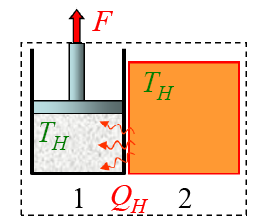
\includegraphics[scale=0.44]{th/image20.png}
\captionof{figure}{Isotherme}
\end{wrapfigure}
Ici $\Delta S = 0$ car l'entropie perdue dans le réservoir vaut celle gagnée dans le gaz. Il s'agit d'une situation \textbf{réversible} (car absence de déséquilibre).

\subsubsection{La détente libre irréversible}
On prend une boîtes à deux compartiment, un vide et un rempli de gaz. On perce un trou entre les deux. L'énergie cinétique reste inchangée car $V' = 2V$ et $P' = P/2$. \\
Cette détente est irréversible, on imagine mal les particules de gaz repasser par le trou pour retrouver la situation initiale.\\

\begin{center}
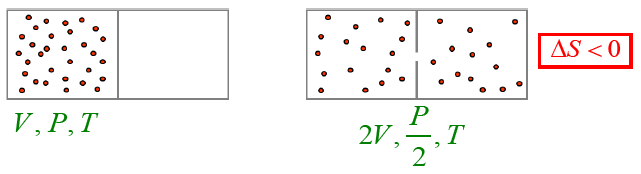
\includegraphics[scale=0.7]{th/image21.png}
\captionof{figure}{Détente libre irréversible}
\end{center}
Cette détente est complexe, mais on ne va considérer que l'état initial et final de sorte à utiliser l'entropie d'une \textbf{isotherme équivalente}.
\begin{equation}
\Delta S = Nk_B\ln\left(\underbrace{\frac{V_f}{V_i}}_{2}\right) > 0
\end{equation}
\subsubsection{Conclusion}
On observera une production d'entropie $\Delta S$ si :
\begin{enumerate}
\item Déséquilibre
\item Irréversibilité
\item Augmentation du désordre
\end{enumerate}
\begin{center}
\fbox{\textit{\textsc{Deuxième principe :} L'entropie d'un système isolé ne peut que rester stable ou augmenter.}}
\end{center}






























\chapter{Électrostatique}
\section{Introduction}
Encore une fois, une bonne lecture attentive suffit !

\section{La force électrique}
\subsection{La force de Coulomb}
Celle-ci a été déterminée à l'aide d'une balance à torsion. Par prise de mesures successive de l'angle fait par le fil en fonction de la charge de la bille, on a pu déterminer les relations de proportionnalités suivantes :
\begin{wrapfigure}[7]{r}{4cm}
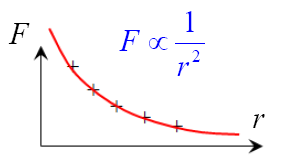
\includegraphics[scale=0.44]{es/image1.png}
\captionof{figure}{Loi de décroissance naturelle}
\end{wrapfigure}
\begin{eqnarray}
F \propto \frac{1}{r^2}\\
F \propto q
\end{eqnarray}
Ces forces ont toujours été obtenues en considérant deux charges. Dès lors :
\begin{equation}
F \propto \frac{q_1q_2}{r^2}
\end{equation}
Pour changer cette proportionnalité en égalité, on définit la constante de Coulomb, $k_0 = 8,987*10^{-9} Nm^2C^{-2}$.
\begin{equation}
\fbox{$ F = k_0 \dfrac{q_1q_2}{r^2}$}
\end{equation}

\subsection{Principe de superposition}
\begin{wrapfigure}[7]{l}{4cm}
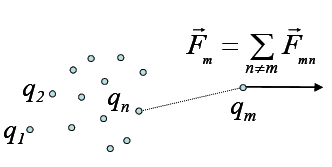
\includegraphics[scale=0.44]{es/image2.png}
\captionof{figure}{Principe de superposition}
\end{wrapfigure}
La convention de signe associée à la force de Coulomb est : $\left\{\begin{array}{l}
+ ; Répulsion\\
- ; Attraction
\end{array}\right.$\\

Notons que la plus petite distance entre les deux charge vaut les deux rayons des charges, sinon l'on aurait une force infinie.\\
La présence d'autre charge n'influent pas sur le résultat :  superposition :
\begin{equation}
\vec{F_m} = k_0\sum_{n\neq m} \frac{q_nq_m}{r^2_{mn}}\vec{1_{r_{mn}}}
\end{equation}

\section{Le champ électrique}
Comme première approche, on peut faire une analogie entre la force électrique $F_e$ et la force gravitationnelle :
\begin{equation}
\vec{F_G} = -C \frac{mm_0}{r^2}\vec{1_r}
\end{equation}
Si la $F_G$ crée un champ gravitationnel, on peut concevoir qu'il en sera de même pour $F_e$. La différence majeure est que $F_e$ peut être positive ou négative.

\subsection{Champ de force}
Il s'agit de l'ensemble des charges que l'on pourrait mesurer dans l'environnement de cette charge sur une deuxième charge mobile (dite "charge d'essai").

\subsection{Champ électrique}
\begin{wrapfigure}[9]{l}{4cm}
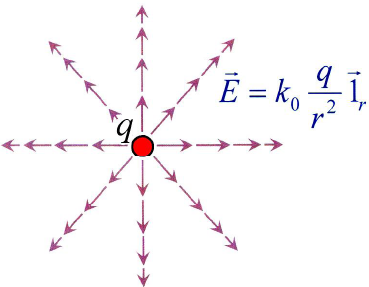
\includegraphics[scale=0.34]{es/image3.png}
\captionof{figure}{Champ électrique}
\end{wrapfigure}
Toujours devoir utiliser deux charges (la charge $q_1$ et la charge d'essai, $q_2$) est très contraignant, c'est pourquoi on passe à la notion de champ qui va caractériser l'environnement indépendamment de la charge d'essai.
\begin{equation}
\fbox{$\vec{E} = \dfrac{\vec{F}}{q} = k_0\dfrac{q}{r^2}\vec{1_r}$}
\end{equation}
L'unité de $E$ sont des $NC^{-1}$. Notons que la force n'a pas toujours le même sens que le champ.


\subsection{Lignes de champ}
\begin{wrapfigure}[9]{r}{6cm}
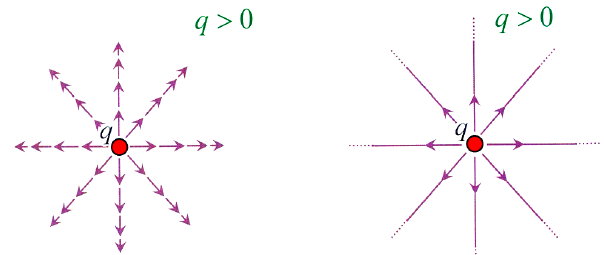
\includegraphics[scale=0.34]{es/image4.png}
\captionof{figure}{Signe du champ}
\end{wrapfigure}
Il s'agit de courbes en tout point tangent au champ électrique. Elles ne donnent en rien la force d'interaction, elles représentent juste le champ (orientation).\\

Celles-ci ne se croisent jamais car un champ ne peut prendre plusieurs valeurs à la fois (car donné de façon univoque par la loi de Coulomb).

\subsection{Champ électrique dans les conducteurs}
\begin{wrapfigure}[7]{l}{5cm}
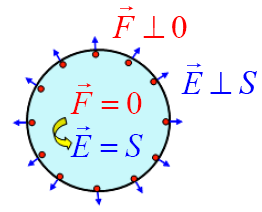
\includegraphics[scale=0.34]{es/image5.png}
\captionof{figure}{Conducteur}
\end{wrapfigure}
Un conducteur est une "substance" qui conduit l'électricité. Leurs électrons (ou ions) peuvent circuler librement.\\
Imaginons un conducteur sphérique. Sa surface peut être vue comme une enceinte de gaz d'électrons libres de se mouvoir. Ajouter des électrons va créer une répulsion, créant un excès de charge positive. Cet excès de charge positive va augmenter jusqu'à avoir compensé exactement la charge négative en excès.\\
Le champ va dès lors se mettre perpendiculairement à la surface à l'équilibre, de façon à ne plus bouger. Si ce n'était pas le cas, les charges se déplacerait et créerait de la chaleur par effet Joule : violerait la conservation d'énergie.\\
L'intérieur d'un conducteur est toujours neutre et le champ est toujours nul.

\subsection{Distribution de charge continue}
\subsubsection{Charges de volume}
Si l'espace est une répartition de charge ponctuelles, on va pouvoir appliquer le principe de superposition.
\begin{equation}
\vec E = k_0 \sum \frac{q_e}{r^2_n}\vec{1_{rn}}
\end{equation}
Il nous faut connaître $r$, la distance entre la charge et le lieu ou l'on calcule le champ. On peut la trouver grâce à la norme (application de Pythagore)\footnote{$(x,y,z)$ sont les coordonnées du point de calcul du champ et $(x_n, y_n, z_n)$ l'emplacement de la charge}
\begin{equation}
r = |\vec{x} - \vec{x_n}| = \sqrt{(x-x_n)^2 + (y-y_n)^2 + (z-z_n)^2}
\end{equation}
Étant l'espace, on va utiliser la densité de charge pour le caractériser : $\rho(\vec{x_n}) = \dfrac{\Delta q_m}{\Delta V_m}$. On peut en tirer $\Delta q = \rho(\vec{x_n)}).\Delta V_m$. En remplaçant dans l'expression du champ et en passant à la limite, on trouve l'expression recherchée.
\begin{equation}
\vec{E}(\vec x) = k_0 \int \frac{\rho(\vec x)}{||\vec{x} - \vec{x'}||^2}\vec{1}_{(x-x')}.dV
\end{equation}

Pour des charges de surface ($\sigma$) et linéique ($\lambda$) le principe est le même ! 


\section{Loi de Gauss}
\subsection{Analogie entre champ électrique et flux de particules}
Une charge ponctuelle émet un flux de photons virtuels (dit "particules", pour ne pas rentrer dans la théorie quantique de l'électromagnétisme).

\subsubsection{Densité de particules}
\begin{wrapfigure}[7]{rl}{5cm}
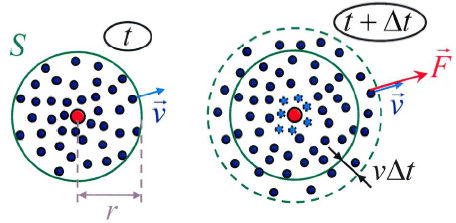
\includegraphics[scale=0.34]{es/image6.png}
\captionof{figure}{Densité de particules}
\end{wrapfigure}
Calculons le flux total à travers une sphère de rayon $r$.
\begin{equation}
\Delta V = \left(\underbrace{4\pi r^2}_{surface}\right) . \underbrace{v.\Delta t}_{épaisseur\ cercle}
\end{equation}
Le nombre de particules s'obtient de la sorte
\begin{equation}
\Delta N = \eta(r).\Delta V
\end{equation}
En remplaçant l'un dans l'autre
\begin{equation}
\Delta N = \eta (r) 4\pi r^2 v\Delta t
\end{equation}
Le flux est le nombre de particules par unité de temps 
\begin{equation}
\Phi = \frac{\Delta N}{\Delta T} = \eta (r) 4\pi r^2 v
\end{equation}
Comme la vitesse est constante, le flux est indépendant de $r$ : pas d'accumulation.\\

Introduisons la \textit{densité de flux de particules}, c'est à dire le nombre de particules traversant une surface par unité de temps : $\vec{F} = \eta (r)\vec{v}$. En isolant :
\begin{equation}
\vec{F} = \eta (r)\vec{v} = \frac{Q}{4\pi r^2}\vec{1_r}
\end{equation}

\subsubsection{Densité de flux}
Insistons sur le fait qu'il s'agit d'une notion locale ! Il faut donc intégrer si l'on veut pour toute la surface.
\begin{equation}
\vec{F} = \frac{Q}{S}\vec{1_r}
\end{equation}
Le flux est constant mais pas $\vec{F}$ qui diminue quand $r$ augmente. On peut voir une ressemblance entre la densité de flux et la charge de Coulomb ($1/r^2$):
$\left\{\begin{array}{l}
\vec{F} = \frac{Q}{4\pi r^2}\vec{1_r}\\
\vec{E} = k_0 \frac{q}{r^2}\vec{1_r}
\end{array}\right.$


\subsection{La permittivité}
Pour des raisons qui apparaîtrons plus tard, posons un changement de variable :
\begin{equation}
k_0 = \frac{1}{4\pi \epsilon_0}
\end{equation}
Recommençons la comparaison : $\left\{\begin{array}{l}
\vec{F} = \frac{q}{4\pi r^2}\vec{1_r}\\
\vec{E} = \frac{q}{4\pi \epsilon_0 r^2}\vec{1_r}
\end{array}\right.$\ \ \ $\Rightarrow\ \ \ \ \dfrac{q}{\epsilon_0} \leftrightarrow \Phi$.

\subsection{Intégrale de flux}
Plutôt que de considérer une sphère, on va s'intéresser à une surface quelconque.
\begin{center}
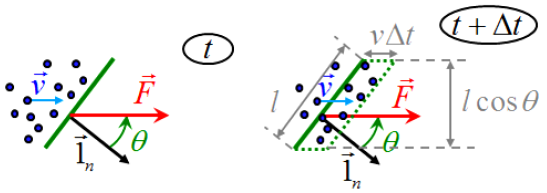
\includegraphics[scale=0.5]{es/image7.png}
\captionof{figure}{Flux à travers d'une surface}
\end{center}
Le nouveau volume parcouru peut être calculé simplement
\begin{equation}
\Delta V = hv\Delta t l \cos\theta = S v \Delta t \cos\theta
\end{equation}
Comme précédemment, $\Delta N = \eta . \Delta V = \eta S v \Delta t \cos\theta$. Nous avons donc comme flux
\begin{equation}
\Phi = \eta v \Delta S_m \cos\theta
\end{equation}
En remarquant l'expression de la densité de flux de particules et la présence d'un produit scalaire, on peut ré-écrire cette expression de façon plus élégante.
\begin{equation}
\Phi_{\Delta_{S_m}} = \vec{F}.\vec{\Delta S_m}
\end{equation}
En sommant toutes ces surfaces élémentaires, on retrouve l'expression du flux à travers toute la surface.
\begin{equation}
\Phi^S = \oint_S \vec{F}(\vec x).d\vec{S}
\end{equation}

\subsection{Flux du champ électrique}
Le résultat obtenu est généralisable pour tout champ vectoriel, y crompsi le champ électrique.
\begin{equation}
\Phi^S_E = \oint_S \vec{E}(\vec{x}).d\vec S
\end{equation}

\subsubsection{Flux au travers d'une surface fermée}
Voyons si ce résultat est cohérent avec l'expression de la densité de flux ($\vec F$)\footnote{Notons qu'ici d$\vec{S}$ étant radial, il vaut $dS.\vec{1_r}$}.\\
\begin{equation}
\Phi = \oint \frac{Q}{4\pi r^2} dS = \Phi\ \ \ \ \ \ \ \ \ \Rightarrow \ \ OK !
\end{equation}
Ce résultat peut être généralisé à toutes surface (si la vitesse est constante).\\
Voyons ce que donne le calcul de cette intégrale. 
\begin{equation}
\oint \vec{E}(\vec x).d\vec{S} = \frac{q}{4\pi r^2 \epsilon_0}\int dS = \frac{q}{\epsilon_0}\ \ \ \ \ \forall\ surfaces !
\end{equation}
Rappelons que cette analogie est possible grâce à la dépendance en $\frac{1}{r^2}$.

\subsubsection{Flux dû à plusieurs charges}
Simple application du principe de superposition
\begin{equation}
\Phi^S_E = \frac{1}{\epsilon_0}\sum_1^N q_n
\end{equation}

\subsubsection{Flux dû à des charges externes}
Tout ce qui va rentrer d'un côté va forcément ressortir de l'autre. Le flux en sera nul ($\Phi = 0$).


\subsubsection{Charges négatives}
Les charges vont "aller" dans l'autre sens, celui opposé à $d\vec S$ : le signe du flux sera négatif. Mais comme la charge sera aussi de signe négatif, les deux moins vont s'annuler et cela ne change au final rien du tout!

\subsubsection{Loi de Gauss}
Ces généralisations étant faites, on peut désormais dire que la Loi de Gauss est généralisée :
\begin{equation}
Loi\ de\ Gauss : \oint_S \vec{E}.d\vec{S} = \dfrac{1}{\epsilon_0}\sum_{m=1}^N q_m
\end{equation}

\subsection{Distributions de charge continue}
Comme vu à la section \textit{3.6}, on peut utiliser $\rho, \sigma\ et\ \lambda$.
\begin{equation}
\Phi^S_E = \oint_S \vec{E}.d\vec{S} = \frac{1}{\epsilon_0}\int_{V_S}\rho(\vec x).dV
\end{equation}

\subsection{Application de la loi de Gauss : calcul de champ}
Voir \textit{Annexe A}, tout y est !
\newpage
\subsection{Forme locale de la Loi de Gauss}
Il s'agit de la version différentielle de la Loi de Gauss : celle-ci appliquée en un point.
\subsubsection{Champ unidirectionnel}
\begin{wrapfigure}[7]{r}{3cm}
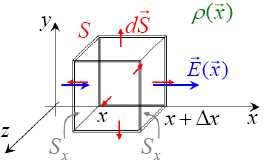
\includegraphics[scale=0.44]{es/image8.png}
\captionof{figure}{Loi de gauss locale}
\end{wrapfigure}
Supposons pour commencer que le champ ne dépend que de $x$ : $\vec{E}(\vec{x}) = \vec{E}(x,y,z) = E_x(x)\vec{1_x}$.\\
Le flux sera ainsi nul pour les autres surfaces. Selon le schéma ci-contre
\begin{equation}
\Phi^S_E = \oint_S \vec{E}.d\vec{S} = \int_{S_x} -E_x(x)ds +  \int_{S_x} E_x(x+\Delta x)dS
\end{equation}
Les surfaces étant infiniment petites, on peut considérer le champ comme constant.
\begin{equation}
-E_x(x)S_x + E_x(x+\Delta x)S_x = \left[E_x(x+\Delta x) - E_x(x)\right].S_x
\end{equation}
Utilisons l'artifice mathématique consistant à multiplier et diviser par $\Delta x$.
\begin{equation}
\Phi^S_E = \left[\frac{E_x(x+\Delta x) - E_x(x)}{\Delta x}\right]\underbrace{S_x\Delta X}_{\Delta V}
\end{equation}
On retrouve ainsi l'expression de la dérivée du champ par rapport à $x$ en faisant tendre $\Delta x \rightarrow 0, \Phi_E^S = \dfrac{dE_x}{dx}\Delta V$.\\
Appliquons la Loi de Gauss
\begin{eqnarray}
\dfrac{dE_x}{dx}\Delta V = \frac{1}{\epsilon_0}\int \rho(\vec x) dV\\
\dfrac{dE_x}{dx}\Delta V =\int \rho(\vec x) \Delta V =
\frac{dE_x}{dx} = \frac{1}{\epsilon_0}\rho(\vec{x})
\end{eqnarray}
Il s'agit la de la loi "locale" car le lien entre $E$ et la densité de charge $\rho$ est donné en un point de l'espace $\vec{x}$.

\subsubsection{Généralisation 3D}
On recommence le même raisonnement pour $x$ et $y$. En mettant tous les résultats ensemble, on obtient la loi de Gauss locale. 
\begin{equation}
\fbox{$\dfrac{\partial E_x(x,y,z)}{\partial x} + \dfrac{\partial E_y(x,y,z)}{\partial y} + \dfrac{\partial E_z(x,y,z)}{\partial z} = \frac{1}{\epsilon_0}\rho(x,y,z)$}
\end{equation}

\subsection{La divergence}
En définissant l'opérateur divergence, $\vec{\nabla}$ on peut noter la loi locale de Gauss sous sa forme compacte.
\begin{equation}
\vec{\nabla}\vec{E} = \frac{1}{\epsilon_0}\rho(\vec x)
\end{equation}
On appelle ceci \textit{divergence} car si le vecteur diverge des élément quittent la surface et le flux en sera positif.
\begin{equation}
\fbox{$div\ \vec{E} = \dfrac{1}{\epsilon_0}\rho(\vec{x})$}
\end{equation}
\textit{La quantité $div\ \vec{E}$ est le flux de particules du champ normalisée (car divisé par sa surface) par le volume défini par la surface fermée captant ce flux.}


\section{Le potentiel électrique}
\subsection{L'énergie potentielle gravitationnelle}
Par définition du travail : $W = F_g.\vec{1_z}\Delta h \rightarrow mg\Delta h$.\\
Par conservation de l'énergie, on peut retrouver la vitesse. En effet : $\frac{1}{2}mv^2 : mgh \Leftrightarrow v = \sqrt{2g\Delta h}$.

\subsection{L'énergie potentielle électrique}
Sa forme est grandement similaire : $W_p(z) = q||\vec{E}||.z (+cste)$. Notons que la force exercée sur la charge est l'opposée de la dérivée de l'énergie potentielle électrique.
\begin{equation}
F_e = - \frac{dW_p}{dz}\vec{1_z}
\end{equation}

\subsection{Potentiel électrique}
Par définition, le potentiel électrique est l'énergie potentielle électrique divisée par la charge.
\begin{equation}
\fbox{$V \equiv \dfrac{W_p}{q_0} = ||\vec E||.z (+cste)$}
\end{equation}
L'unité du potentiel est le Volt ($V$).

\subsection{Potentiels de champs non-uniformes}
On décompose la trajectoire en déplacement infinitésimaux. Le travail élémentaire correpondant au déplacement nous intéressant est donné par le produit scalaire de la force $\vec{F_a}$ (l'inverse de la force électrique que subit la charge, c'est à dire $-qE$) par le vecteur déplacement $\vec{dl}$.
\begin{center}
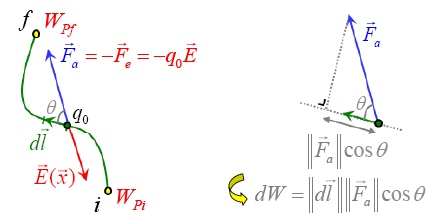
\includegraphics[scale=0.6]{es/image9.png}
\captionof{figure}{Décomposition infinitésimale de la trajectoire}
\end{center}
Comme $W = F.L$, en tenant compte de l'angle (et en passant à l'infinitésimal) : $dW = ||\vec{dl}||.||\vec{F}||.\cos\theta = \vec{F}.\vec{dl} = -q\vec{E}.\vec{dl}$.\\
Comme $V = \frac{W}{q}$ :
\begin{equation}
\Delta V = - \int_{i \rightarrow f} \vec{E}.\vec{dl}
\end{equation}

\subsection{Potentiel coulombien}
Nous savons que : $\left\{\begin{array}{l}
\vec{E} = \frac{q}{q\pi \epsilon_0 r^2}\vec{1_r}\\
\Delta V = - \int_{i \rightarrow f} \vec{E}.\vec{dl}
\end{array}\right.$. Injectons l'un dans l'autre :
\begin{equation}
\Delta V = -\frac{q}{4\pi \epsilon_0}\int_{r_i}^{r_f} \frac{dr}{r^2}
\end{equation}
L'idée du potentiel coulombien est de faire venir une charge de l'infini ($r_i = \infty$), c'est à dire quand on ne "ressent" plus les effets de la charge. Ce qui donne, après intégration\footnote{Souvent utilisé en pratique : $W = qV(r)$}
\begin{equation}
V(r) = \frac{q}{4\pi \epsilon_0 r}
\end{equation}
Il s'agit d'un champ scalaire (et non vectoriel comme $\vec{F}$ et $\vec E$).\\
Rappelons qu'on travail négatif signifie que la charge se fait attirer, c'est à dire qu'elle \textit{reçoit} de l'énergie.

\subsubsection{Chemin quelconque}
\begin{wrapfigure}[6]{l}{5.5cm}
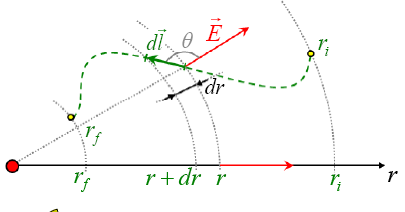
\includegraphics[scale=0.44]{es/image10.png}
\captionof{figure}{Chemin quelconque}
\end{wrapfigure}
On remarque grâce au schéma ci-contre que $\vec{E}.\vec{dl} = ||\vec{E}||.||\vec{dl}||.\cos\theta = ||\vec{E}||.dr$.\\
La trajectoire est identique à celle radiale.\\

Le potentiel est donc indépendant du chemin suivi, ce qui implique que la force électrique est conservative.\\
\ \\

\subsection{Potentiel dû à plusieurs charge}
On applique encore et toujours le principe de superposition !
\begin{equation}
\Delta V = \sum_1^N \Delta V_n
\end{equation} 

\subsubsection{Potentiel du dipôle}
Les calculs se trouvent dans le syllabus, voici ici le résultat compte-tenu de l'approximation du premier-ordre.
\begin{equation}
V(x) \approx \frac{q}{4\pi \epsilon_0}\frac{xd}{r^3}
\end{equation}

\subsection{Potentiel d'une distribution de charges continue}
Même principe que précédemment. Par exemple, pour $\rho$ :
\begin{equation}
V(x) = \frac{1}{4\pi \epsilon_0}\int\frac{\rho (x')}{||x-x'||}dV'
\end{equation}

\subsection{Le moment dipolaire}
Par analogie au centre de masse et au moment (\textit{Cf. mécanique rationelle I}), le moment dipolaire est défini par
\begin{equation}
\vec{p} = \int \rho (\vec{x}).x'.dV
\end{equation}
Un autre résultat (souvent utilisé en pratique) est : 
\begin{equation}
\vec{p} = Q_+ <x_n^+> - Q_-<x_n^->
\end{equation}

\newpage
\subsection{Moment de force sur un dipôle}
Un couple de force s'appliquant sur une "barre" n'a qu'un seul effet possible : causer un déplacement en rotation (du au moment de force, \textit{Cf. ConFond, Meca I}).

\begin{center}
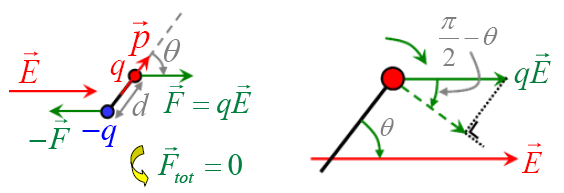
\includegraphics[scale=0.6]{es/image11.png}
\captionof{figure}{Couple de force et bras de levier}
\end{center}
Plus l'angle $\theta$ est petit, plus l'effet sera faible.  La composante de cette force en $x$ vaut $q.E\cos(\frac{\pi}{2} - \theta) = qE\sin\theta$.\\
Connaissant la définition du moment de force $\tau$ (\textit{bras de levier * force $\perp$, $\tau = d.F_\perp$}) nous avons : \\
\begin{equation}
\tau = d.q.E\sin\theta
\end{equation}
En travaillant avec des demi-bras de levier ($\frac{d}{2}$) et en les sommant, on trouve
\begin{equation}
\tau = qE\frac{d}{2}\sin\theta + qE\frac{d}{2}\sin\theta
\end{equation}
Ce que l'on peut ré-écrire (vectoriellement ici, par propriété du produit vectoriel)
\begin{equation}
\vec{\tau} = qd\vec{1_p}\times \vec{E}
\end{equation}
En posant $\vec p = qd\vec{1_p}$ on trouve l'expression générale du moment de force sur un dipôle.
\begin{equation}
\fbox{$\vec{\tau} = \vec{p} \times \vec{E}$}
\end{equation}

\subsubsection{Généralisation}
On retombe exactement sur le même résultat en passant par la décomposition infinitésimale ($\tau = \int d\tau$).\\
Ce sont les dipôles qui explique l'alignement des molécules d'eau dans le même sens.

\subsection{Détermination du champ électrique à partir du potentiel}
Partons de la relation bien connue donnant le potentiel en fonction du champ et dérivons la.
\begin{equation}
\Delta V = - \int_{i\rightarrow f} \vec{E}.\vec{dl}\ \ \ \ \Rightarrow\ \ \ \ dV = - \vec{E}.\vec{dl}
\end{equation}
Qu'est ce que $dV$ ? Il s'agit d'un déplacement infinitésimal 
\begin{equation}
dV = \frac{\partial V(x,y,z)}{\partial x}dx + \frac{\partial V(x,y,z)}{\partial y}dy + \frac{\partial V(x,y,z)}{\partial z}dz
\end{equation}
Connaissant le vecteur $\vec{dl} = dx\vec{1_x} + dy\vec{1_y}+dz\vec{1_z}$, on voit que l'on peut écrire $dV$ comme le produit scalaire suivant :
\begin{equation}
dV = \vec{\nabla}V.\vec{dl}
\end{equation}
Pour rappel : 
\begin{equation}
\vec{\nabla} \equiv \frac{\partial}{\partial x}\vec{1_x} + \frac{\partial}{\partial y}\vec{1_y} + \frac{\partial}{\partial z}\vec{1_z} \Rightarrow \vec{\nabla}V \equiv \frac{\partial V}{\partial x}\vec{1_x} + \frac{\partial V}{\partial y}\vec{1_y} + \frac{\partial V}{\partial z}\vec{1_z}
\end{equation}
On remarque que $\vec{\nabla}.\vec{dl}$ donne la même expression que $dV$
\begin{equation}
\vec{\nabla}.\vec{dl} = \frac{\partial V(x,y,z)}{\partial x}dx + \frac{\partial V(x,y,z)}{\partial y}dy + \frac{\partial V(x,y,z)}{\partial z}dz
\end{equation}
Dès lors, on peut dire que 
\begin{equation}
\vec{\nabla}V.\vec{dl} = -\vec{E}.\vec{dl}\ \ \ \ \Rightarrow\ \ \ \ \vec{E} = - \vec{\nabla}V
\end{equation}
L'opérateur $\vec{\nabla}$ est aussi appelé \textit{gradient}.
\begin{equation}
\fbox{$\vec{E} = -grad\ V$}
\end{equation}

\subsubsection{Interprétation du gradient}
Le gradient donne la direction de la plus grande pente positive.

\section{Capacité électrique}
\subsection{Générateur de Van de Graff}
\begin{wrapfigure}[10]{r}{3cm}
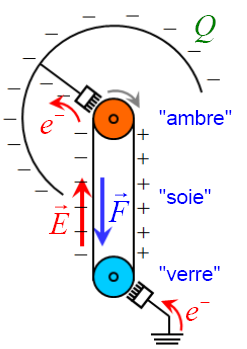
\includegraphics[scale=0.34]{es/image12.png}
\captionof{figure}{Générateur de Van de Graff}
\end{wrapfigure}
On remarque que plus on charge la sphère, plus le champ électrique augmente. Plus celui-ci est fort, plus la force électrique est importante. Forcément, le travail nécessaire pour ajouter une nouvelle charge est plus conséquent.\\
On remarque ainsi un lien de proportionnalité :
\begin{equation}
W \propto Q
\end{equation}
Rappelons que les charges se répartissent selon une densité surfacique de sorte que le champ soit chaque fois perpendiculaire à la surface.

\subsection{Capacité électrique}
Comme $W \propto Q$ et que $V = \frac{W}{q}$ on peut dire que $V \propto Q$. En introduisant un coefficient de proportionnalité $Q$, la capacité électrique, on définit l'égalité suivante :
\begin{equation}
\fbox{$Q = CV$}
\end{equation}

\subsection{Capacité de la sphère}
Grâce à la loi de Gauss, on peut trouver le champ d'une sphère 
\begin{equation}
\Phi = 4\pi r^2 ||\vec{E}|| = \frac{q}{\epsilon_0}\ \ \ \ \Rightarrow\ \ \ \ E = \frac{q}{4\pi \epsilon_0 r^2}
\end{equation}
Le potentiel associé à ce champ vaut 
\begin{equation}
V_{sphère} = \frac{q}{4\pi \epsilon_0 r}
\end{equation}
Or, $Q = CV\ \ \rightarrow\ \ V = \frac{Q}{C}$. Par comparaison, on trouve que la capacité de la sphère vaut :
\begin{equation}
C_{sphère} = 4\pi \epsilon_0 r
\end{equation}
Si la capacité $C$ augmente, le travail $W$ diminue et plus on pourra rajouter de nouvelles charges facilement. Ainsi, plus $C$ est grand, plus la différence de potentiel sera réduite.

\subsection{Énergie de la charge}
On apporte à une sphère des petites charges infinitésimales $dq$. Le travail nécessaire pour apporter ces charges vaut $V.q = V(q).dq$
\begin{equation}
W = \int_0^q V(q).dq = \int_0^q \frac{q}{C}dq = \frac{q^2}{2} 
\end{equation}
Comme $Q = CV$, on retrouve l'expression faisant l'objet de tous vos fantasmes :
\begin{equation}
\fbox{$W_e = \dfrac{CV^2}{2}$}
\end{equation}
Notons que l'unité de la capacité électrique est le $Farad, F$.


\subsection{Capacité électrique et influence électrostatique}
\begin{wrapfigure}[12]{l}{3.5cm}
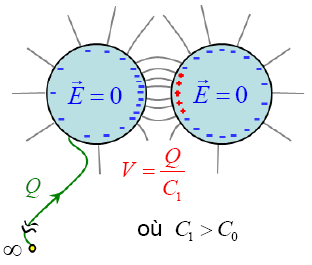
\includegraphics[scale=0.44]{es/image13.png}
\captionof{figure}{Influence électrostatique}
\end{wrapfigure}
Plus on charge, par exemple, une sphère, plus le travail nécessaire augmente. Il est intéressant de pouvoir augmenter la capacité.\\
En approchant une deuxième sphère non chargée, celle-ci va subir la répulsion des charges négatives et l'attraction des charges positives. Il s'agit de l'\textbf{influence électrostatique}.\\
Les lignes de champ sont plus denses entre les deux sphères, le champ à donc obligatoirement diminué dans les zones plus éloignée de l'entre-deux sphère (résultat découlant de la Loi de Gauss).\\
Comme il existe des endroit ou apporter des charges est plus simple, on peut dire que le potentiel à diminué et donc, la charge étant constante ($C = Q/V$), la capacité électrique a augmenté.\\ Si l'on connecte la deuxième sphère au sol, elle gagne une capacité infinie et la capacité de notre première sphère se voit encore augmentée. Notons qu'à l'équilibre, les charges seront égales mais opposée : c'est le principe du \textbf{condensateur}.

\subsection{Le condensateur électrique plan}
\begin{wrapfigure}[12]{r}{3.5cm}
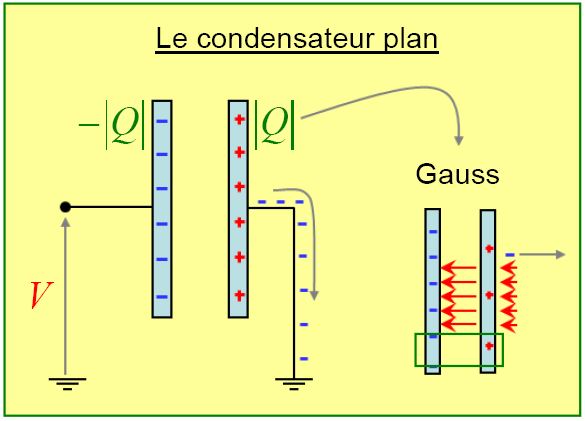
\includegraphics[scale=0.24]{es/image14.png}
\captionof{figure}{Condensateur plan}
\end{wrapfigure}
Le principe est le même, mais la géométrie est plus simple.  La justification du champ nul à l'équilibre s'obtient en prenant une surface de Gauss cylindrique contenant les deux plans de charges. Le flux est négatif mais par influence électrostatique il diminue en valeur absolue jusqu'à devenir nul.\\
A l'équilibre, le flux est nul et le champ extérieur l'est également : ils ne subissent plus de force de coulomb.\\
La condition d'équilibre est d'avoir une charge globale nulle.

\subsection{Calcul de la capacité du condensateur plan}
Nous avons connaissance du champ d'une plaque seule\footnote{Que si le plan est considéré comme infini et que l'on calcule le champ loin des bords}
\begin{equation}
\vec{E}_{plaque} = \frac{\sigma}{\epsilon_0}\vec{1_S}
\end{equation}
Pour utiliser cette relation, on va considérer le plan infini pour négliger les distorsions des lignes de champs aux extrémités. \textbf{Hypothèses : $h, l >> e$}.\footnote{$e$ est la distance entre les deux plaques}

\begin{wrapfigure}[19]{l}{6cm}
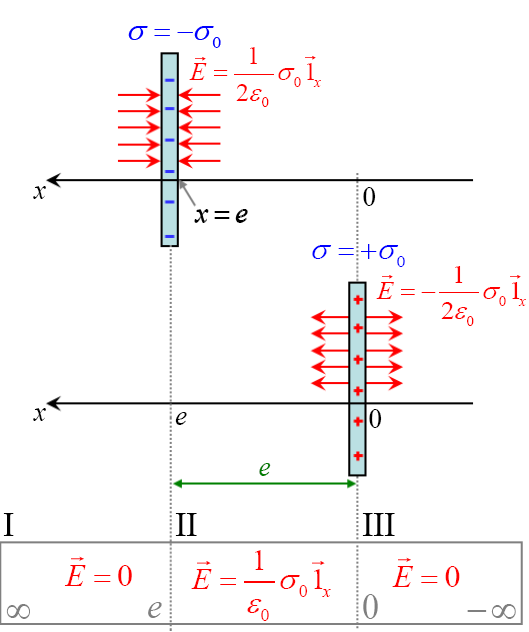
\includegraphics[scale=0.44]{es/image15.png}
\captionof{figure}{Condensateur plan}
\end{wrapfigure}
Calculons le champ grace au principe de superposition : on considère le champ généré par chaque plaque et l'on somme les résultats.\\
La plaque de gauche a une charge négative, son champ sera dès lors attractif. L'autre plaque sera donc chargé positivement et aura un champ répulsif.\\
On remarque qu'en dehors de l'entre-deux plaques, le champ est nul (les lignes de champ se compensent).
\begin{equation}
E_{cond_{ext}} = 0
\end{equation}

Par contre, entre les deux plaque, le champ est doublé et vaut
\begin{equation}
\fbox{$\vec{E}_{cond} = \dfrac{\sigma}{\epsilon_0}\vec{1_x}$}
\end{equation}
Notons que tant que les deux plaques ne sont pas à l'équilibres, des électrons sont poussés à l'extérieur.\\


Le champ du condensateur étant connu, calculons sa capacité électrique. Nous savous que $V = - \int \vec{E}.\vec{dl}$ où $E = \frac{\sigma}{\epsilon_0}$.
\begin{equation}
V = -\frac{\sigma}{\epsilon_0}\int_0^e dx = -\frac{\sigma e}{\epsilon_0} \overbrace{=}^{Q = -\sigma S} = \frac{Qe}{\epsilon_0 S}
\end{equation}
Sachant que $C = \frac{Q}{V}$ on trouve
\begin{equation}
\fbox{$C_{cond} = \dfrac{\epsilon_0 S}{e}$}
\end{equation}
C'est donc l'épaisseur $e$ qui détermine l'influence électrostatique. Plus elle est petite, plus l'influence sera grande et la capacité sera élevée.

\subsection{Milieux diélectriques et polarisation}
On peut encore augmenter la capacité électrique en incorporant un milieu non-conducteur, dit \textit{conducteur diélectrique}. \textbf{Hypothèse :} le milieu diélectrique est constitué d'une juxtaposition d'atomes identiques.
\begin{center}
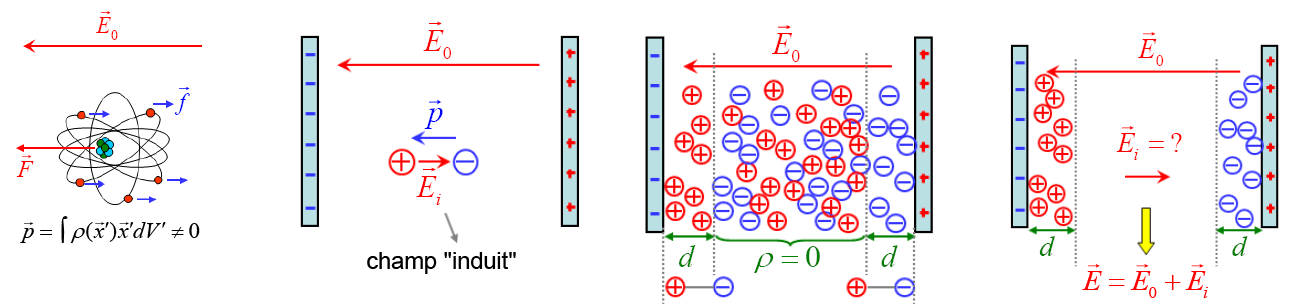
\includegraphics[scale=0.48]{es/image16.png}
\captionof{figure}{Champ induit du au milieu diélectrique}
\end{center}
Le champ électrique du condensateur va causer une légère déformation de l'atome, qui va acquérir un moment dipolaire (\textsc{Figure 2.16.1})\\
On constate l'apparition d'un champ électrique induit qui s'oppose au champ extérieur (généré par les deux plaques) (\textsc{Figure 2.16.2}).\\

Les atomes du diélectrique ne peuvent se rapprocher à une distance inférieure à $d$ : formation d'une pellicule chargée d'épaisseur $d$ responsable d'une diminution du champ total (polarité inversée) (\textsc{Figure 2.16.3}).\\

Le champ total peut dès lors s'écrire (\textsc{Figure 2.16.1}) :
\begin{equation}
\vec{E} = \vec{E_0} + \vec{E_i}
\end{equation}
Comment calculer le champ induit $\vec{E_i}$ ? On sait que l'épaisseur $d$ sera proportionnelle au champ $E$. En introduisant la \textit{déformabilité $\alpha$}, on peut dire que $d = \alpha E$. Le moment dipolaire $\vec{p} = d.\vec{F}$ vaut donc :
\begin{equation}
\vec{p} =: \alpha q\vec{E}
\end{equation}
Connaissant $\left\{\begin{array}{l}
\eta = \frac{Q}{S}\\
Q = V.\rho = \eta_a q d s
\end{array}\right.$ on peut dire que $\sigma = \eta_a q d = \eta_a q \alpha E$ où $E = \frac{\sigma}{\epsilon_0}$.
Le champ induit vaut donc\footnote{Signe négatif car toujours opposé à $E_0$} :
\begin{equation}
E_i = -\frac{\eta_a q \alpha E}{\epsilon_0}
\end{equation}
En introduisant la susceptibilité $\chi\ \ \Rightarrow\ \ \vec{E_i} = -\chi \vec{E}$.\\
Mais que vaut $\vec{E}$? Sachant que $\vec{E} = \vec{E_0} + \vec{E_i} = \vec{E_0} - \chi \vec{E} \Leftrightarrow \vec{E}(1+\chi) = \vec{E_0}$\\
Le champ total $\vec{E}$ peut être calculé :
\begin{equation}
\fbox{$\vec{E} = \dfrac{\vec{E_0}}{(1+\chi)}$}
\end{equation}

Le champ rempli d'un diélectrique est donc plus faible d'un facteur $(1+\chi)$, où $E_0$ est le champ du condensateur vide (= sans diélectrique). D'autres éléments doivent être modifier pour tenir compte du di-électrique :
\begin{eqnarray}
V &=& \frac{V_0}{(1+\chi)}\\
C &=& (1+\chi)\frac{\epsilon_0 S}{e}\\
 &=& \epsilon \frac{S}{e}\ où\ \epsilon\ =\ permittivité : \epsilon_0(1+\chi)\\
\epsilon_r &=& \frac{\epsilon}{\epsilon_0} = 1+\chi
\end{eqnarray}

\subsection{Le condensateur en pratique}
\textit{Voir annexe A}

\subsection{Énergie stockée}
Même chose que précédemment (conservation d'énergie)
\begin{equation}
W_e = \frac{CV^2}{2}
\end{equation}
\subsubsection{Densité d'énergie électrique}
Le but est d'exprimer l'énergie stockée en fonction du champ sachant  que
\begin{equation}
\left\{\begin{array}{l}
W = \frac{CV^2}{2}\\
V = e\vec{E}\\
C = \frac{\epsilon_0 S}{e}
\end{array}\right.
\end{equation}
On peu en tirer que 
\begin{equation}
w = \frac{1}{2}\epsilon||E||^2
\end{equation}


\section{Résistance électrique}
\subsection{Définition du courant}
\begin{wrapfigure}[7]{l}{6cm}
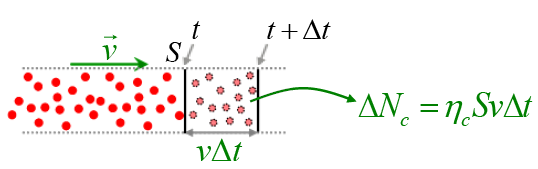
\includegraphics[scale=0.44]{es/image17.png}
\captionof{figure}{Courant électrique}
\end{wrapfigure}
Le courant est un flux de charges électriques 
\begin{equation}
\fbox{$I \equiv \dfrac{\Delta q}{\Delta t}$}
\end{equation}
Le nombre de particules sur un temps $\Delta t$ vaut : $\Delta N =  \eta S v\Delta t$. On multiplie par la charge d'une particules pour avoir la charges : $\Delta q = \eta q_e S v\Delta t$\\
Connaissant la définition du courant $I$, on trouve ce-dernier.
\begin{equation}
I = \eta q_e vS
\end{equation}
L'unité du courant électrique est l'ampère ($A$).\\
\textbf{Attention !} Le sens du courant descend le potentiel (d'où $E = -grad\ V$) \textit{mais} les électrons remontent le potentiel (à cause de leur signe négatif...).

\subsection{Densité de courant}
On utilise souvent en pratique la notion de densité de courant. Il s'agit du courant divisé par la surface.
\begin{equation}
J = \frac{I}{S}= \eta e_e v
\end{equation}
On écrit souvent $\vec{J}$ sous sa force vectorielle. Son sens est toujours le même que celui du champ. \\
Une expression très utilisée en pratique est l'expression du courant sous sa forme intégrale que voici :
\begin{equation}
I = \int_S \vec{J}.d\vec{S}
\end{equation}

\subsection{Source de tension continue : la pile électrique}
Le champ va du $+ \rightarrow -$, mais les électrons font l'inverse.

\subsection{La conduction électrique}
L'accélération des électrons augmente l'énergie cinétique et donc la température. 
\begin{equation}
\vec{v_m} = -\mu \vec{E}
\end{equation}
où $\mu$ est la mobilité et $\vec{v_m}$ la vitesse moyenne des électrons.

\subsection{Forme locale de la loi d'Ohm}
On part de la densité de courant $\vec{J} = \eta q \vec{v}$ où $\vec{v} = -\mu \vec{E}$.\\
On peut ré-écrire $\vec{J} = \eta q \mu \vec{E}$. On pose $\sigma = \eta q \mu$ comme étant le conductivité et l'on tombe sur la loi d'Ohm locale.
\begin{equation}
\fbox{$\vec{J} = \sigma\vec{E}$}
\end{equation}

\subsection{Loi d'Ohm}
$I = ||\vec{J}||.S$ et $\left\{\begin{array}{l}
I = \sigma S ||\vec{E}||\\
||\vec{E}|| = \frac{V}{L}
\end{array}\right.$\ \ \ $\Rightarrow\ \ \ I = \frac{\sigma S V}{L}$ où $\frac{L}{\sigma S} \equiv R$, la résistance électrique.\\
On retrouve la loi d'Ohm, bien connue en secondaire.
\begin{equation}
\fbox{$V = RI$}
\end{equation}
L'unité de la résistance est l'Ohm, $\Omega$.

\subsection{Les résistances}
On définit la résistivité comme étant l'inverse de la conductivité : $\rho_e = \frac{1}{\sigma_e}$.
\begin{equation}
R = \frac{L}{\sigma_e S} = \frac{\rho_e L}{S}
\end{equation}

\subsubsection{Le potentiomètre}
Permet de diviser la tension.

\subsubsection{Association de résistance}
\textit{Cf. Annexe A}

\subsection{Puissance dissipée : effet Joule}
\begin{wrapfigure}[10]{l}{3cm}
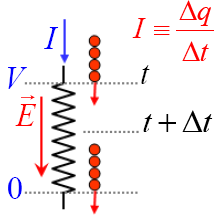
\includegraphics[scale=0.44]{es/image18.png}
\captionof{figure}{Puissance dissipée}
\end{wrapfigure}
Toute la charge qui rentre vaut celle qui sort : il y a \textit{conservation de la charge}. La différence de potentiel d'un fil est nulle $\Delta V_{fil} = 0$ car la résistance du fil est nulle ($V = RI$).\\

Dans une résistance, la diminution de l'énergie potentielle ne se converti pas en énergie cinétique (car la vitesse est fixée, $\vec{v_m} = -\mu \vec{E}$) mais en chaleur : transfert collisionnel.\\
L'énergie potentielle (chute de potentiel) est donc convertie en chaleur ! Calculons le travail :
\begin{equation}
\Delta W = V.\Delta q = VI \Delta t
\end{equation}
La puissance étant $P = \frac{\Delta W}{\Delta t}$ :
\begin{equation}
\fbox{$P = IV$}
\end{equation}
Comme V = RI, plusieurs expression de la puissance dissipée peuvent être trouvées :
\begin{equation}
P = RI^2 = \frac{V^2}{R} = IV
\end{equation}
Une résistance à température constante (= à régime) dissipe un débit de chaleur $H = IV$.

\subsection{Circuit RC}
\subsubsection{Décharge du condensateur}
\begin{wrapfigure}[6]{l}{4.5cm}
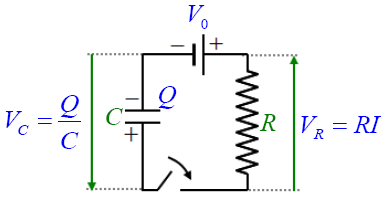
\includegraphics[scale=0.44]{es/image19.png}
\captionof{figure}{Circuit RC}
\end{wrapfigure}
On a tout d'abord besoin d'une résistance (comme une turbine qui diminue l'$E_C$ pour fournir un $W$) dite "utile" $\rightarrow$ résistance de charge. Nous avons :\\
$\left\{\begin{array}{l}
V = \frac{Q}{C}\\
V = RI\\
I = -\frac{dQ}{dt}
\end{array}\right.$\ \ \ $\Rightarrow\ \ RI = \frac{Q}{C}$.\\
En passant à l'expression différentielle
\begin{wrapfigure}[6]{r}{3cm}
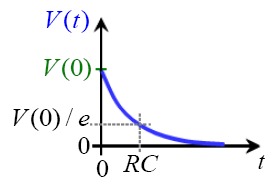
\includegraphics[scale=0.44]{es/image20.png}
\captionof{figure}{Décharge du RC}
\end{wrapfigure}
\begin{equation}
\frac{dQ}{dt} = - \frac{Q}{RC}
\end{equation}
Résolvons l'équation différentielle de premier ordre.
\begin{eqnarray}
\frac{dQ}{Q} &=& -\frac{dt}{RC}\\
\ln (Q) &=& \frac{t}{RC} + C\\
Q &=& Q(0).e^{-\frac{t}{RC}}
\end{eqnarray}

Cette équation différentielle exprime la vitesse ou la charge s'écoule, proportionnellement aux charges restantes dans le condensateur. On peut également trouver le potentiel associé :
\begin{equation}
V(t) = V(0).e^{-\frac{t}{RC}}
\end{equation}
\subsubsection{Charge du condensateur}
Le principe est le même, si ce n'est que l'équation différentielle n'est pas homogène.
\begin{equation}
\frac{dQ}{dt} = -\frac{Q}{RC} + \frac{V_0}{R}
\end{equation}
Le cours d'\textit{Analyse I} nous donne la S.G.E.H et la solution particulière. La Solution Générale de l'Equation Non-Homogène (S.G.E.N.H.) est la suivante (\textit{Cf. Syllabus + Analyse I})
\begin{equation}
V_C(t) = V_0\left(1 - e^{-\frac{t}{RC}} \right)
\end{equation}
\begin{center}
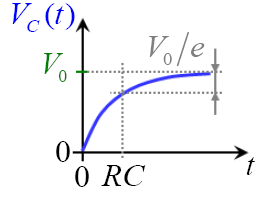
\includegraphics[scale=0.6]{es/image21.png}
\captionof{figure}{Charge du condensateur}
\end{center}


\tableofcontents
\end{document}

